\documentclass{article}
\usepackage[francais]{babel}
\usepackage[utf8]{inputenc}  
\usepackage{listings}
\usepackage{graphicx}
\usepackage{color}
\usepackage{float}
\usepackage{algorithm}
\usepackage{algorithmic}
\usepackage{caption}

\usepackage{array}
\usepackage{colortbl}
\usepackage{amsfonts}
\usepackage{geometry}
\usepackage{setspace}
\usepackage{hyperref}
\usepackage{subcaption}
\usepackage{listings}

\newcolumntype{P}[1]{>{\centering\arraybackslash}p{#1}}
\newcolumntype{M}[1]{>{\centering\arraybackslash}m{#1}}

\definecolor{mygreen}{rgb}{0,0.6,0}
\definecolor{gray}{rgb}{0.5,0.5,0.5}
\definecolor{mymauve}{rgb}{0.58,0,0.82}
\definecolor{backcolour}{rgb}{0.95,0.95,0.92}

\lstset{ 
  language=fortran,
  backgroundcolor=\color{backcolour},   
  basicstyle=\footnotesize,        % the size of the fonts that are used for the code
  captionpos=b,                    % sets the caption-position to bottom
  commentstyle=\color{mygreen},    % comment style
  deletekeywords={...},            % if you want to delete keywords from the given language
  escapeinside={\%*}{*)},          % if you want to add LaTeX within your code
  keepspaces=true,                
  keywordstyle=\color{blue},       % keyword style
  otherkeywords={*,...},           % if you want to add more keywords to the set
  numbers=left,                   
  numbersep=5pt,                   % how far the line-numbers are from the code
  numberstyle=\tiny\color{gray}, % the style that is used for the line-numbers
  rulecolor=\color{black},        
  showspaces=false,               
  showstringspaces=false,          % underline spaces within strings only
  showtabs=false,                  % show tabs within strings adding particular underscores
  stepnumber=1,                    % the step between two line-numbers. If it's 1, each line will be numbered
  stringstyle=\color{mymauve},     % string literal style
  tabsize=2,	                   % sets default tabsize to 2 spaces
  title=\lstname                   % show the filename of files included with \lstinputlisting; also try caption instead of title
}

\makeatletter
\renewcommand\thesection{}
\renewcommand\thesubsection{\@arabic\c@section.\@arabic\c@subsection}

\makeatother


\addto\captionsfrench{\def\refname{Bibliographie}}
\begin{document}

\begin{titlepage}
  \centering
  \begin{minipage}[t]{0.48\textwidth}
    \begin{flushleft}
      
\includegraphics[width=0.85\textwidth]{figures/logo_fac.jpg}\par\vspace{0.5cm}
      \begin{spacing}{1.5}
%        \textsc{\LARGE Université de ...}
      \end{spacing}
    \end{flushleft}
  \end{minipage}
  \begin{minipage}[t]{0.48\textwidth}
    \begin{flushright}
      
\includegraphics[width=0.8\textwidth]{figures/logo_cerfacs.eps}\par\vspace{0cm}
 %     \textsc{\LARGE Entreprise}
    \end{flushright}
  \end{minipage} \\[1.5cm]


  % {\scshape\LARGE Université de Bordeaux \par}
  % \vspace{1cm}
  {\scshape\LARGE Stage de fin d'étude\par}
  \vspace{1.5cm}
  {\huge\bfseries Simulation numérique directe de la combustion turbulente\par}
  \vspace{2cm}
  {\Large\itshape Adrien Guilbaud\par}
  \vfill
  Maître de stage\par
  Mme.~Isabelle \textsc{D'ast}
  \vspace{0.5cm}

  Enseignant responsable\par
 
  Mr.~Samuel \textsc{Thibault}

  \vfill

  % Bottom of the page
  {\large Année universitaire 2015-2016\par}
\end{titlepage}

\null\cleardoublepage
\section*{Résumé}\addcontentsline{toc}{section}{Résumé}
Lorem ipsum dolor sit amet, consectetur adipiscing elit, sed do eiusmod tempor incididunt ut labore et dolore magna aliqua. Ut enim ad minim veniam, quis nostrud exercitation ullamco laboris nisi ut aliquip ex ea commodo consequat. Duis aute irure dolor in reprehenderit in voluptate velit esse cillum dolore eu fugiat nulla pariatur. Excepteur sint occaecat cupidatat non proident, sunt in culpa qui officia deserunt mollit anim id est laborum.
\null\cleardoublepage
\section*{Remerciements}%\addcontentsline{toc}{section}{Remerciements}
Je tiens tout d'abord à remercier l'ensemble des enseignants de la spécialité Calcul Haute Performance de l'université de Bordeaux et de l'ENSEIRB pour la formation reçue qui m'a fournie les connaissances nécessaires pour ce stage.

\paragraph{}Je remercie également l'ensemble des équipes CSG et CFD avec lesquelles j'ai pu travailler durant ce 6 mois de stage pour leur acceuil généreux.

\paragraph{}Je remercie tout particulièrement Isabelle D'AST pour l'aide qu'elle m'a apporté tout au long de ce stage ainsi que pour son soutien durant ces longues heures de débogage/fous rires nerveux. Je remercie également Bénédicte CUENOT pour m'avoir guidé sur la partie physique nécessaire à la bonne compréhension de ce stage même si la CFD gardera ses mystères ("\textit{un front de flamme c'est comme de la mayonnaise}").

\null\cleardoublepage
\tableofcontents
\null\clearpage

\listoffigures  % table des figures
\listoftables   % table des tableaux
\null\cleardoublepage
\section{Introduction}
\subsection{Le Cerfacs}\label{sec:intro}

Le Cerfacs (Centre Européen de Recherche et de Formation Avancée en Calcul Scientifique) est un centre de recherche spécialisé dans le calcul scientifique et la simulation numérique. Créé en 1987, il travaille pour ses actionnaires (Airbus Group, Cnes, EDF, Météo France, Onera, Safran et Total) à la résolution de problèmes scientifiques et techniques liés au climat, à l'aéronautique, au spatial et à l'environnement par la simulation numérique nécessitant une puissance de calcul élevée. Il travaille également en partenariat avec le CNRS, l'Irit, le CEA ainsi que l'Inria.


Le personnel du Cerfacs est réparti en équipes:
\begin{itemize}
\item Algorithmes parallèles
\item Aviation \& environnement
\item Informatique et Support Utilisateur (CSG)
\item Modélisation du climat
\item Mécanique des fluides (CFD)
\end{itemize}

\subsubsection{L'équipe CFD}
L'équipe CFD (\textit{Computational Fluid Dynamics: mécanique des fluides numérique}) est la plus grosse équipe du Cerfacs et c'est en son sein que j'ai réalisé mon stage. Elle se concentre sur le développement de méthodes numériques permettant la simulation des écoulements et les applique aux avions, fusées, moteurs, turbines, etc. Ces méthodes permettent ensuite d'étudier les mouvements de fluides et leurs effets par la résolution d'équations régissant de tels fluides. L'avantage des simulations mises en place est grand pour l'industrie; elles permettent d'étudier des phénomènes complexes pour un coût très inférieur à des expériences réelles.

Bénédicte CUENOT, une des chef de projet de l'équipe, m'encadrait pour la partie physique de mon stage.


\subsubsection{L'équipe CSG}
L'équipe CSG (\textit{Computer Support Group}) s'occupe de la gestion des infrastructures informatiques et des moyens matériels mis à la disposition des différentes équipes. Elle fournit également son expertise aux chercheurs pour qu'ils puissent exploiter au mieux les outils et le matériel disponibles.
Dans le cadre de mon stage, j'ai surtout eu contact avec Mme Isabelle D'AST, ingénieur Logiciel HPC. C'est elle qui m'a conseillé sur toute la partie HPC (\textit{High Performance Computing}) et plus généralement, sur tous les problèmes liés à la programmation.

\subsection{Le stage}
\subsubsection{NTMIX\_CHEMKIN}
Mon stage portait sur NTMIX\_CHEMKIN, un des codes de simulation développé par l'équipe CFD. C'est un solveur d'écoulements réactifs (``écoulements dans lesquels il y a des réactions chimiques'') en 2D s'appuyant sur une approche DNS (Direct Numerical Simulation). Il est couplé avec la librairie CHEMKIN qui permet la simulation de la chimie complexe. Ce code est utilisé pour étudier la structure chimique des flammes et leur comportement en présence d'un écoulement dynamique (combustion turbulente).\cite{cerfacs}



Une simulation numérique directe (DNS: Direct Numerical Simulation) est une simulation dans laquelle les équations de Navier-Stokes (équations décrivant le mouvement des fluides visqueux) sont résolues numériquement sans aucun modèle de turbulence. Cependant, le coût d'une telle simulation est très élevé. Il est actuellement impossible de résoudre des problèmes industriels avec ce type de simulation. Elle présente cependant un intérêt en recherche fondamentale. Grâce à la DNS, il est possible de faire des ``expériences numériques'' et d'en extraire des informations difficilement récupérables en laboratoire.\cite{cfd-online-DNS}


\subsubsection{Objectifs}
Comme vu précedemment, le coût d'une simulation réalisée par NTMIX\_CHEMKIN est très élevé. Son utilisation était donc restreinte au cas en bidimensionnel, mais l'évolution des machines de calcul parallèle permet aujourd'hui d'utiliser une version tridimensionnelle à des coûts raisonnable.


Le développement d'une version 3D est motivé par le fait que NTMIX\_CHEMKIN utilise une librairie permettant de prendre en compte les cinétiques complexes des éléments chimiques (CHEMKIN), contrairement à NTMIX\_3D, un autre logiciel de simulation développé au Cerfacs, déjà en 3D mais n'utilisant pas de chimie complexe. Le portage en 3D permettra donc d'observer des phénomènes complexes ne pouvant pas forcément être obtenus avec d'autres méthodes de simulation.


Cependant, une simulation DNS n'utilise pas de modèle de turbulence. Il sera nécessaire de paralléliser la version 3D de NTMIX\_CHEMKIN pour permettre au code de traiter de grands maillages ($\approx 10^9$ points) en un temps raisonnable.


\paragraph{}Pour atteindre ces objectifs, il sera nécessaire de procéder par étapes; dans un premier temps, j'ai dû moderniser le code avant de développer une version 3D de celui-ci. Cette partie a permis d'obtenir une première version tridimensionnelle, testée et validée de NTMIX utilisant des concepts de programmation plus récents et sera présentée en section \ref{sec:part1}

Dans la section \ref{sec:part2}, je me suis intéressé au développement d'une version parallèle de l'application et aux modifications induites par une telle version. Cette version devra permettre d'exécuter des simulations sur des machines parallèles.

Enfin, dans une dernière partie (section \ref{sec:part3}), je mesurerai les performances de NTMIX sur les calculateurs internes du Cerfacs afin d'essayer de tirer les meilleurs performances possibles.

\paragraph{}A terme, la version finale de NTMIX permettra de faciliter la compréhension de phénomènes complexes liés à la mécanique des fluides et pourra aboutir à la rédaction de publications scientifiques par les chercheurs en combustion du Cerfacs.

\subsection{Présentation de la mécanique des fluides}
\subsubsection{Mécanique des fluides numérique}
La \textbf{mécanique des fluides} est l'étude du comportement des fluides (liquides, gaz et plasma) lorsqu'ils sont en mouvement et est un domaine actif de recherche notamment en mécanique des fluides numérique (\textit{ou CFD}). Ce sous-domaine s'intéresse à l'étude des mouvements par la \textbf{résolution numérique} des équations régissant les fluides. Les équations les plus utilisées sont:

\begin{itemize}
\item les équations d'Euler dans le cas des fluides parfaits; elle ne prennent pas en compte la viscosité et la conductivité thermique
\item les équations de Navier-Stokes dans le cas des fluides newtoniens
\end{itemize}


Dans NTMIX, ce sont les équations de Navier-Stokes; équations aux dérivées partielles qui sont résolues.

Cependant, la mécanique des fluides numérique se base sur des versions discrétisées de ces équations. Pour NTMIX, le domaine de calcul (espace) est divisé en volumes élémentaires (discrétisation spatiale) selon une approche structurée (maillage structuré) qui consiste à découper l'espace en cellules régulièrement espacées selon toutes les directions du domaine.


\subsubsection{Simulation de la turbulence}
Dans un écoulement turbulent, des tourbillons instables apparaissent à toutes les échelles et interagissent entre eux. Pour pouvoir simuler un tel comportement, il existe 3 approches différentes:

\begin{itemize}
\item la méthode de simulation directe (\textit{DNS: Direct Numerical Simulation}): elle consiste à utiliser un maillage plus fin que le plus petit tourbillon attendu (fig. \ref{fig:dns})
\item la simulation des grandes échelles (\textit{LES: Large Eddy Simulation}): un modèle de turbulence est utilisé pour les plus petits tourbillons, permettant ainsi d'utiliser un maillage plus grossier (fig. \ref{fig:les})
\item la simulation de l'écoulement moyen statistique (\textit{RANS: Reynold Averaged Navier-Stokes Simulation})
\end{itemize} 


\begin{figure}[ht]
  \centering
  \begin{subfigure}[b]{0.5\textwidth}
    \centering
    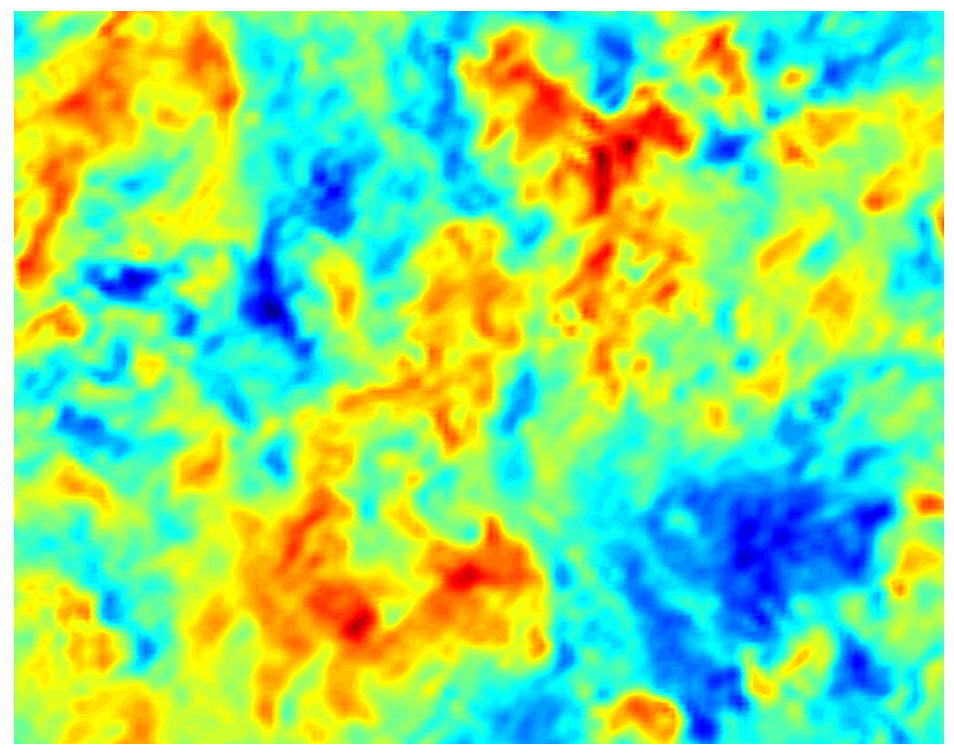
\includegraphics[scale=0.35]{figures/DNS_Velocity_Field.png}
    \caption{\label{fig:dns} Simulation des turbulences (DNS)}
  \end{subfigure}%
  ~
  \begin{subfigure}[b]{0.5\textwidth}
    \centering
    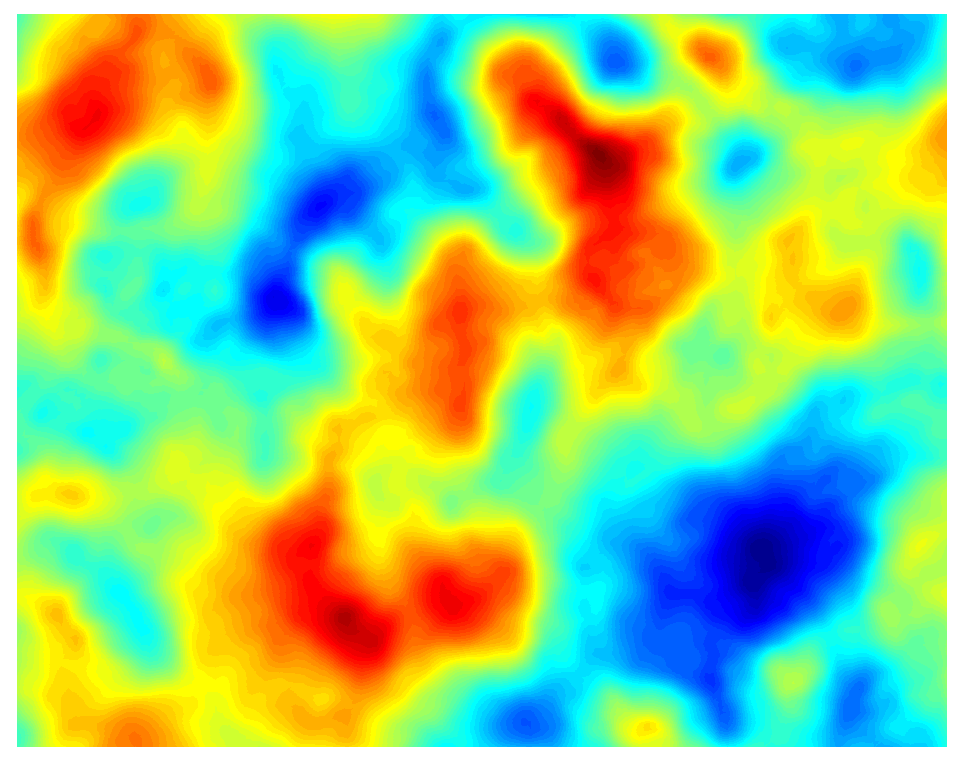
\includegraphics[scale=0.35]{figures/DNS_Filtered_Velocity_Field_Large.png}
    \caption{\label{fig:les} Simulation des grandes turbulences (LES)}
  \end{subfigure}
\end{figure}

L'approche DNS est donc la plus coûteuse en terme de puissance de calcul nécessaire étant donné qu'aucun modèle de turbulence n'est utilisé contrairement à la méthode LES qui ne simule que les tourbillons les plus grands, les petits tourbillons étant seulement modélisés. Les domaines d'applications de ces différentes méthodes sont donc différents; l'approche DNS est plutôt réservée à la recherche du fait des coûts élevés de telles simulations tandis que les méthodes LES et RANS sont plus adaptées à un contexte industriel.


\subsubsection{Vocabulaire lié à la CFD}

\begin{itemize}
\item Variables conservatives: ce sont les variables utilisées dans la simulation et qui sont soumises aux lois de conservation; conservation de masse, énergie et quantité de mouvement. Les variables conservatives se rapporteront donc ici à la masse volumique, l'énergie et les vitesses selon toutes les directions.
\item Champ: c'est l'association d'une valeur d'un paramètre à un point de l'espace ou du maillage. Il existe des \textbf{champs scalaires} qui associent une valeur (masse volumique, pression, etc.) à chaque point et des \textbf{champs vectoriels} qui associent un vecteur (vitesses) à chaque point de l'espace.
\item Gradient: c'est une opération réalisée sur un champ. C'est une généralisation de la dérivée pour une fonction à plusieurs variables.

\end{itemize}

\cleardoublepage
\section{Partie 1: Migration de NTMIX en Fortran 90 et développement d'une version 3D}

Avant de commencer à développer une version en 3 dimensions de NTMIX, j'ai dû moderniser le code. En effet, NTMIX a été développé en Fortran 77 ce qui ne permettait pas l'allocation dynamique de tableau; l'ensemble des variables étaient allouées de manière statique ce qui augmentait grandement la taille de l'executable. Pour résoudre ce problème et permettre plus de flexibilité, il m'a été demandé de migrer le code du standard Fortran 77 au standard Fortran 90.
% Le programme devait donc être entièrement recompilé à chaque changement de la taille du maillage.

\subsection{Migration de NTMIX}
\subsubsection{Travail réalisé}

\paragraph{Réécriture de code}Cette partie consistait donc à réécrire le code dans une norme plus récente. Une majorité des modifications était liée à la syntaxe du code. Pour rendre la tâche plus aisée, j'ai utilisé des expressions régulières; ce sont des séquences de caractères qui définissent des motifs de recherche et qui sont particulièrement utiles pour remplacer un motif par un autre. Par exemple, en Fortran 77, le C ou c placé en début de ligne indique le début d'un commentaire mais en Fortran 90 c'est un ! qui a cet usage. La figure \ref{fig:regex} montre une expression utilisée pour modifier ces commentaires dans le code; ils sont très nombreux et on peut donc automatiser la tâche. 

\begin{figure}[ht]
  \centering
  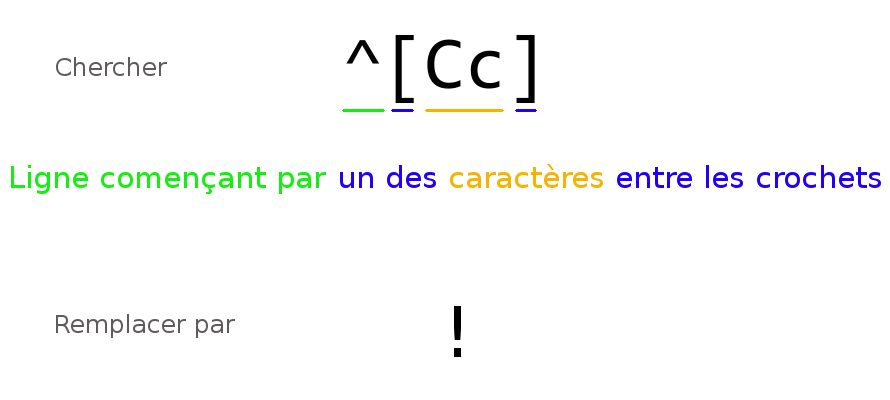
\includegraphics[scale=0.3]{figures/regex.png}
  \caption{\label{fig:regex}Exemple d'expression régulière}
\end{figure}

%Exemple ^#.*?"\(.*?\)\.com"

\paragraph{Gestion de la mémoire}En Fortran, les blocs COMMON permettent de définir des zones mémoires globales, accessible depuis n'importe où dans le code. Le problème est qu'il faut répliquer ce bloc à chaque endroit du code où les variables qu'il contient doivent être utilisées, le plus souvent avec des instructions non-standard du Fortran. Un autre problème est qu'il faut définir la taille des tableaux contenus dans ces blocs à la compilation, ce qu'y va à l'encontre de mon objectif. Pour palier à ces problèmes, ces blocs ont été transformés en modules (introduits en Fortran 90) qui permettent également d'avoir une zone de mémoire globale mais les tailles des tableaux peuvent être précisées à l'exécution.

\paragraph{Post-traitement}NTMIX génère des fichiers binaires contenant l'état physique de la simulation à un instant donnée. Un programme annexe à NTMIX permettait de transformer ces fichiers en fichiers pouvant être visualisés grâce à Plot3D. Ce code ne fonctionnant plus, je l'ai modifié pour qu'il génère des fichiers HDF5 (Hierarchical Data Format) qui permettent de structurer de grandes quantités de données. Cependant, ces fichiers ne peuvent être directement lus par un logiciel de visualisation, j'y ai donc joint des fichiers XDMF (eXtensible Data Model and Format). Ce format a été développé pour le calcul haute performance et notamment pour permettre la visualisation des données par des logiciels comme ParaView ou EnSight en autorisant la définition d'un maillage auquel joindre les données.


\begin{figure}[ht]
  \centering
  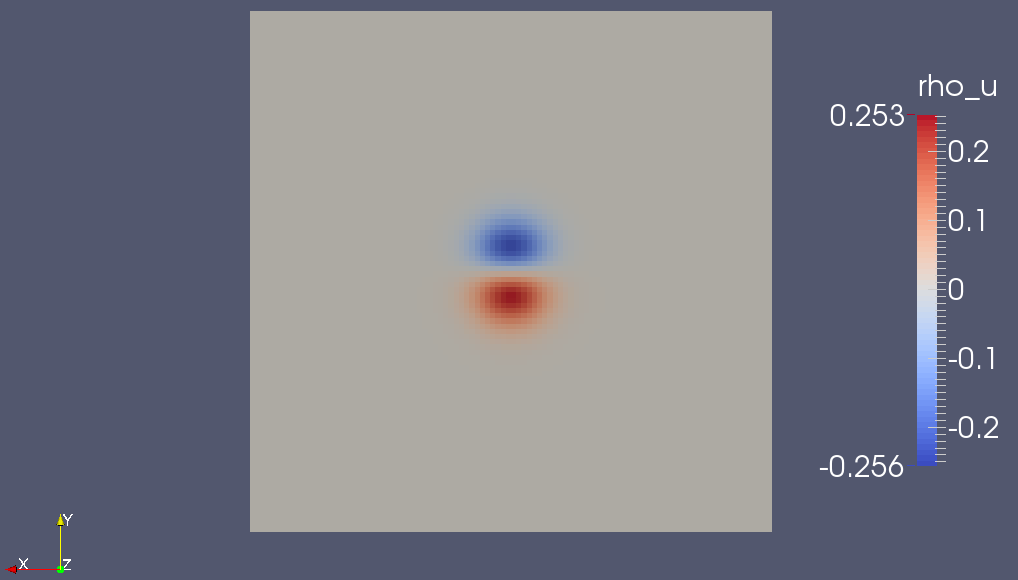
\includegraphics[scale=0.3]{figures/vertex.png}
  \caption{\label{fig:visu}Exemple de visualisation - ParaView TODO:THI}
\end{figure}

%\begin{itemize}
%\item Changement de syntaxe
%\item Changement des bloc commom en modules
%\item Changement des equivalence en pointeur
%\item Allocation dynamique des tableaux
%\item Utilisation de namelist pour changer la taille du maillage et certains paramètres du problème physique.
%\end{itemize}


\subsubsection{Validation}Pour vérifier que les modifications réalisées ne changeaient pas le comportement du programme, j'ai écrit un script permettant de comparer les résultats fournis par ma version avec ceux du programme initial. NTMIX lit la configuration physique de la simulation depuis des fichiers d'entrée. Le script génère donc ces fichiers avec plusieurs configuration, lance la version initiale, la version en cours de développement puis compare les solutions calculées par ceux-ci.

\paragraph{}J'ai également utilisé Valgrind, un outil permettant notamment d'analyser la mémoire d'un programme afin de vérifier que la mémoire allouée dynamiquement était toujours désallouée, évitant ainsi l'apparition de fuites mémoire (pouvant entrainer une saturation de la mémoire de la machine ainsi qu'un plantage du code).




\subsection{Passage en 3D}

\subsubsection{Méthode}\label{sec:3dmeth}
Dans cette partie, je me suis intéressé au passage de l'application en 3 dimensions. Pour minimiser les erreurs pouvant être induites par ce changement, j'ai modifié le code par petits blocs. Une grande partie des variables conservatives (densité, vitesses, énergie..) sont stockées dans un seul tableau et des pointeurs viennent délimiter ce tableau en sous-tableaux (fig. \ref{fig:array_2d}). Ces pointeurs représentaient tous des tableaux 2D. J'ai donc dans un premier temps modifié la taille du grand tableau pour qu'il puisse contenir la dimension supplémentaire mais en laissant les pointeurs aux bons emplacements et j'ai ajouté des tableaux 3D, qui n'étaient pas encore utilisés à ce moment-là. A partir de là, j'ai remplacé progressivement les tableaux 2D par les tableaux 3D en vérifiant que les résultats restaient identiques au fur et à mesure. Cette méthode m'a donc permis de réduire le risque d'erreurs au maximum.

\paragraph{Calcul des gradients}Après avoir réalisé ces modifications, je me suis intéressé aux calculs des gradients. Ils indiquent la façon dont les grandeurs physiques (densité, vitesse, énergie, etc.) évoluent au cours du temps. Ces calculs s'effectuaient sur un plan; il a donc fallu les modifier pour qu'il prennent en compte tout l'espace.

\paragraph{Conditions limites}Une simulation DNS doit être très précise et ne fournit pas de moyen de minimiser la création d'ondes d'instabilités numérique qui se propagent ensuite dans le domaine, sont réfléchies aux frontières et peuvent générer de nouvelles ondes physiques\cite{baritaud1996direct}. Pour palier à ce problème, la méthode NSCBC(Navier-Strokes Characteristic Boundary Conditions) est utilisé dans NTMIX. J'ai donc dû implémenter la version 3D de cette méthode à l'aide des équations fournies par Poinsot et Lele (1992)\cite{POINSOT1992104}

\paragraph{}Plusieurs parties du code prévoyait déjà le passage du code en 3 dimensions, ainsi la préparation des tableaux utilisés pour le calcul des gradient était présente et a facilité le travail. La librairie CHEMKIN est adimensionnée ce qui a permis d'ajouter une dimension sans avoir à modifier ses fonctions.

%\begin{itemize}
%\item Changement de la taille des tableaux
%\item Ajout de la vitesse sur l'axe Z
%\item Ajout des conditions limites sur Z
%\item Modification du calcul des dérivées
%\item Modification du calcul de l'énergie cinétique: $\rho_e = \rho\frac{1}{2}(u^2+v^2+w^2)$
%\end{itemize}

\subsubsection{Validation}
Comme dit dans précedemment (sec. \ref{sec:3dmeth}), j'ai d'abord testé le comportement du programme 3D en précisant une dimension nulle ce qui m'a permis de comparer les résultats avec la version 2D. J'ai ensuite mis en place plusieurs tests 3D permettant de valider les calculs réalisés par le programme:

\begin{itemize}
\item Écoulements uniformes: un flux uniforme traverse le domaine selon un axe; le flux étant constant, les dérivées doivent rester nulles et les vitesses ne doivent pas varier
\item Un front de flamme est une zone dans laquelle se déroule la combustion:
  \begin{itemize}
  \item Vitesse nulle: le front de flamme doit rester statique et un phénomène de diffusion doit être observé (mouvement de molécules d'une région de haute concentration vers une région de faible concentration)
  \item Vitesse non-nulle: en plus du phénomène de diffusion, la convection doit également apparaitre (mouvement de groupe de molécules au sein d'un fluide)
  \end{itemize}
\item Turbulence homogène isotrope
\end{itemize}

\paragraph{Écoulements uniformes}
Comme dit précédemment, les dérivées doivent être nulles dans ce cas, la simulation doit donc rester dans son état initial. Comme on peut le voir sur la figure \ref{fig:uniform_flow}, les vitesses selon les 3 axes sont restées constantes au cours du temps.
 
\begin{figure}[ht]
  \centering
 % \includegraphics[scale=0.3]{figures/uniform_flow.png}
  \caption{\label{fig:uniform_flow}Flot uniforme}
\end{figure}

\paragraph{Front de flamme}
Un cas simple a été utilisé pour ce front de flamme; 2 espèces chimique et la concentration d'une espèce est modélisée par une gaussienne centrée simplifiée en $e^{-(x^2)}$ et l'autre par $1-e^{-(x^2)}$ permettant ainsi d'avoir une concentration de 1 en tout point du domaine. Pour observer l'effet de diffusion, nous utilisons la fonction dérivée d'une gaussienne: $f(x,t)=\frac{1}{t}e^{f}$. Sur la figure \ref{fig:diff}, nous pouvons observer en bleue la valeur initiale d'une espèce, en vert sa valeur au temps $t$ de la simulation et en rouge la valeur théorique.

% $f(x,t_0)=e^{\frac{-(x-x_0)^2}{\sigma^2}}$
%\begin{figure}[ht]
%  \centering
%  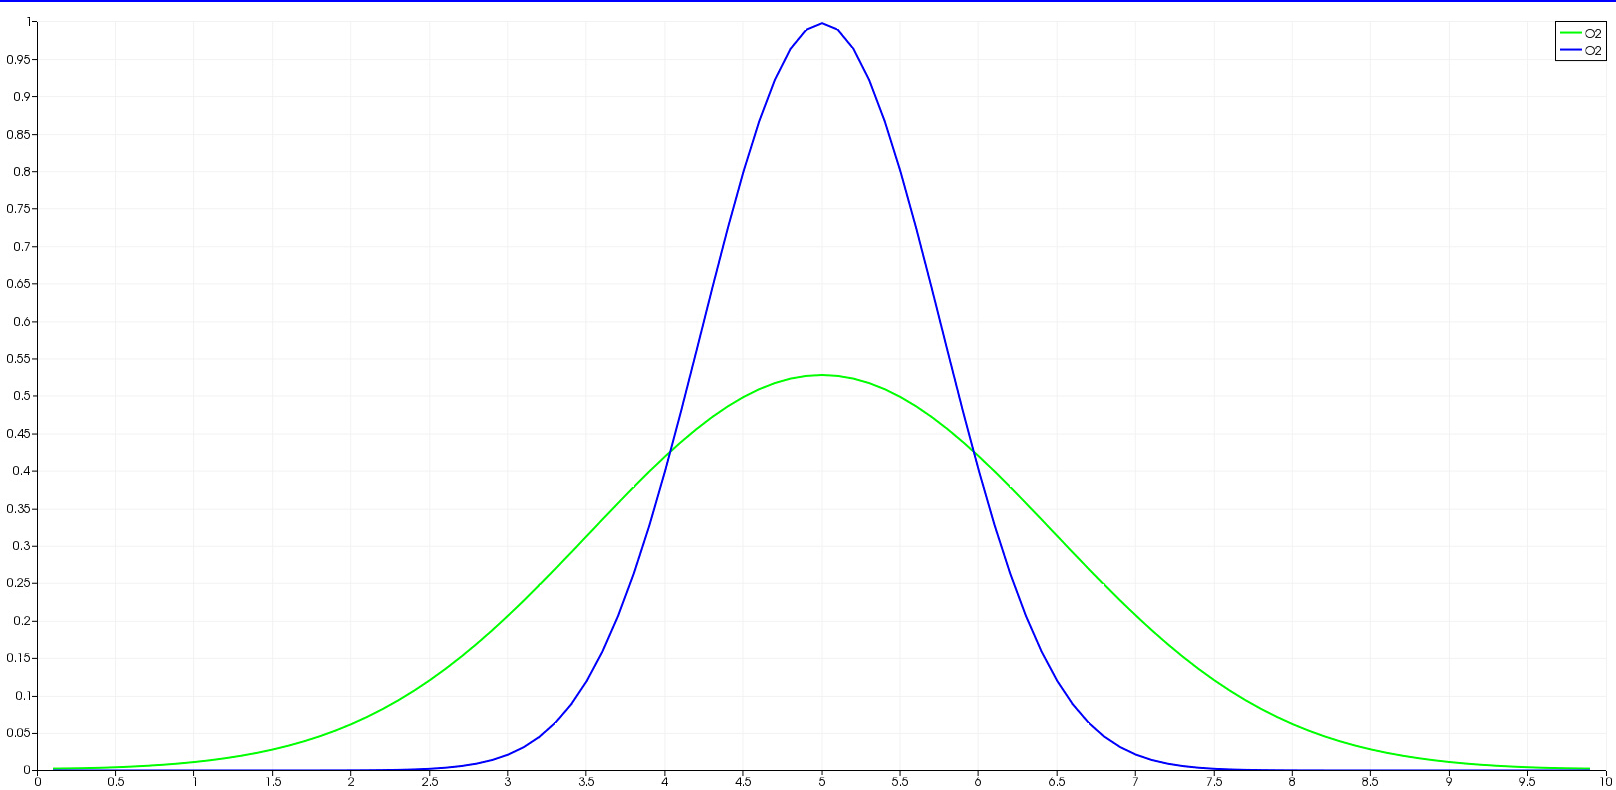
\includegraphics[scale=0.15]{figures/diff.png}
%  \caption{\label{fig:diff} }
%\end{figure}

\begin{figure}[t!]
  \centering
  \begin{subfigure}[b]{0.5\textwidth}
    \centering
    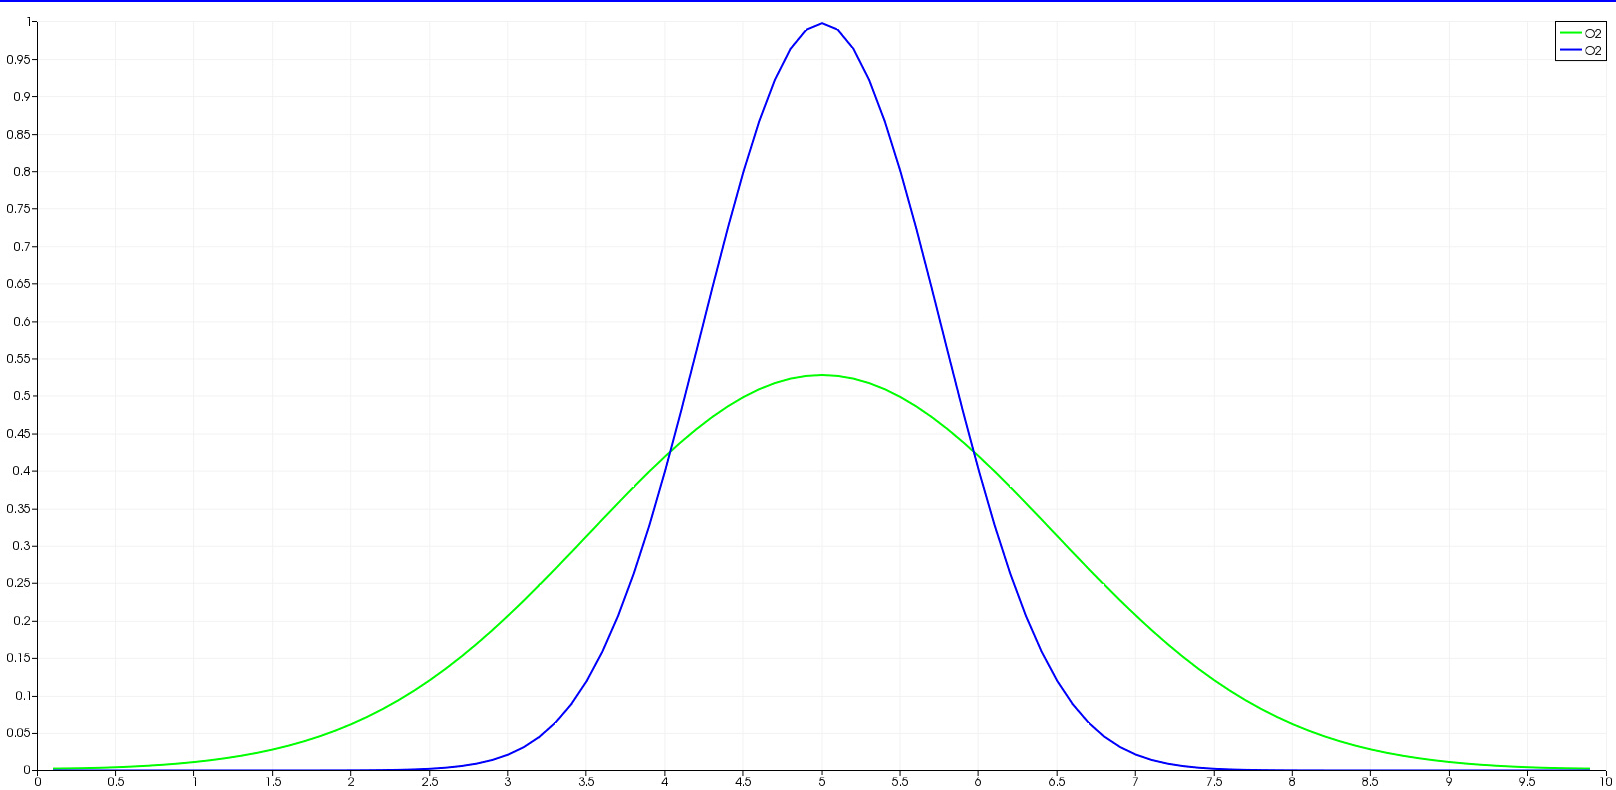
\includegraphics[width=.9\linewidth]{figures/diff.png}
    \caption{\label{fig:diff_0}Valeur x $t_0$}
  \end{subfigure}%
  ~ 
  \begin{subfigure}[b]{0.5\textwidth}
    \centering
    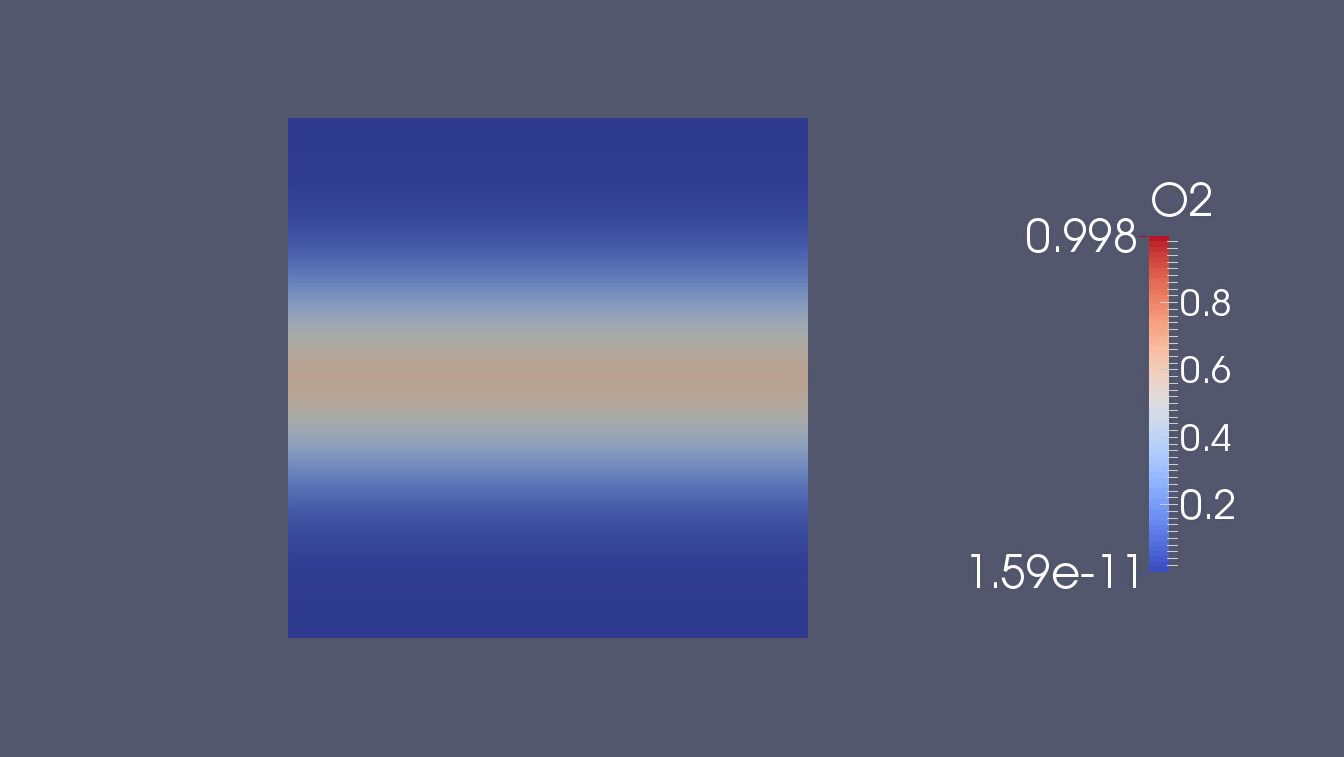
\includegraphics[width=.9\linewidth]{figures/diff_325.png}
    \caption{\label{fig:diff_325}Valeur x $t$}
  \end{subfigure}
  \caption{Caption place holder}
  \centering
  \begin{subfigure}[b]{0.5\textwidth}
    \centering
    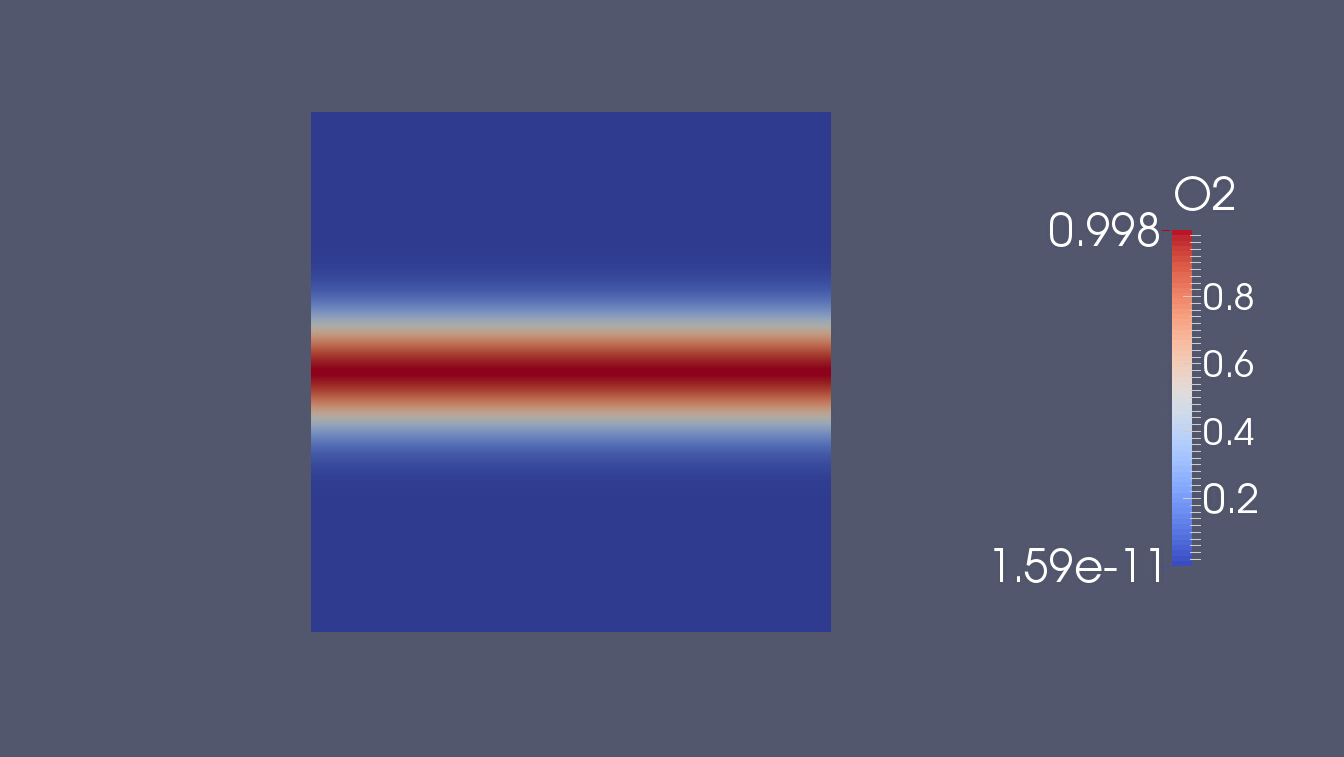
\includegraphics[width=.9\linewidth]{figures/diff_0.png}
    \caption{\label{fig:diff_0_domain}Valeur x $t_0$ - Domaine complet}
  \end{subfigure}%
  ~ 
  \begin{subfigure}[b]{0.5\textwidth}
    \centering
    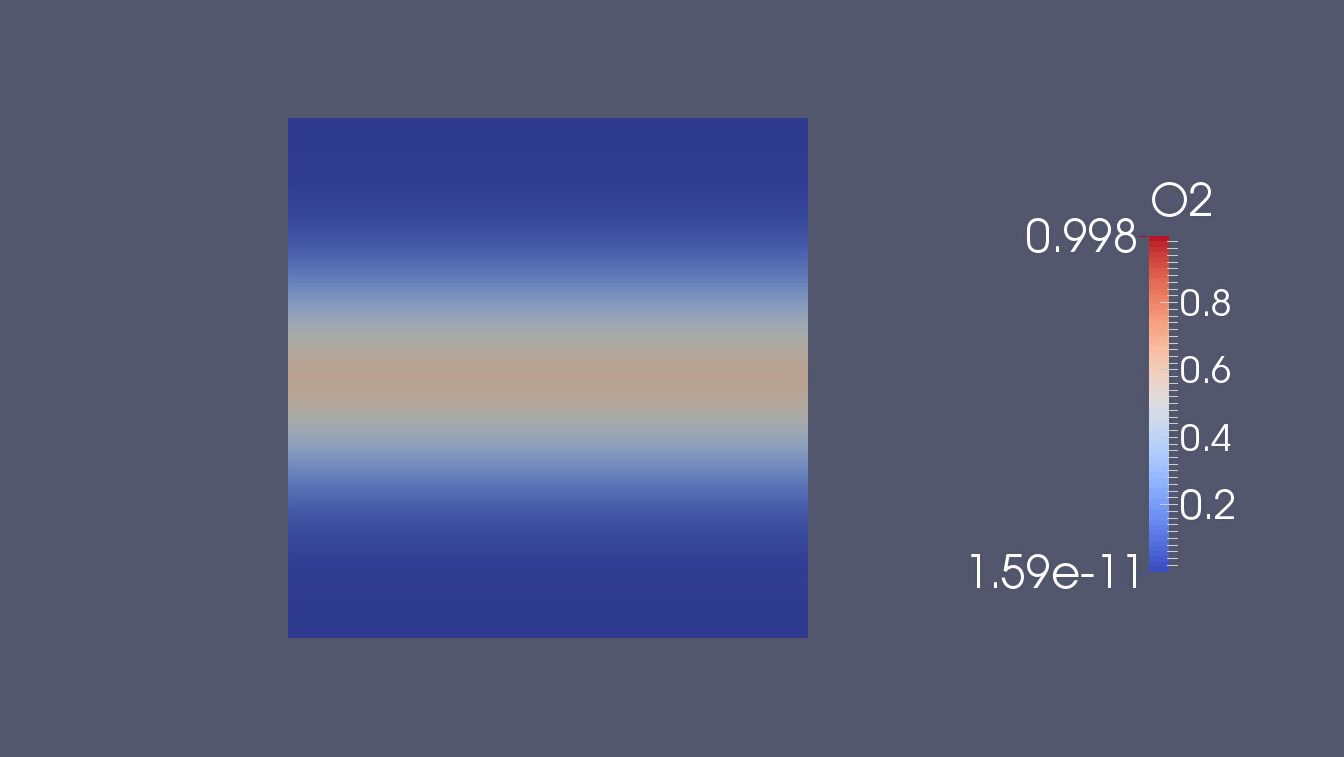
\includegraphics[width=.9\linewidth]{figures/diff_325.png}
    \caption{\label{fig:diff_325_domain}Valeur x $t$ - Domaine complet}
  \end{subfigure}
  \caption{\label{fig:diff_}Diffusion}
\end{figure}


%\begin{figure}[ht]	
%  \centering
%  \begin{minipage}{.5\textwidth}
%    \centering
%    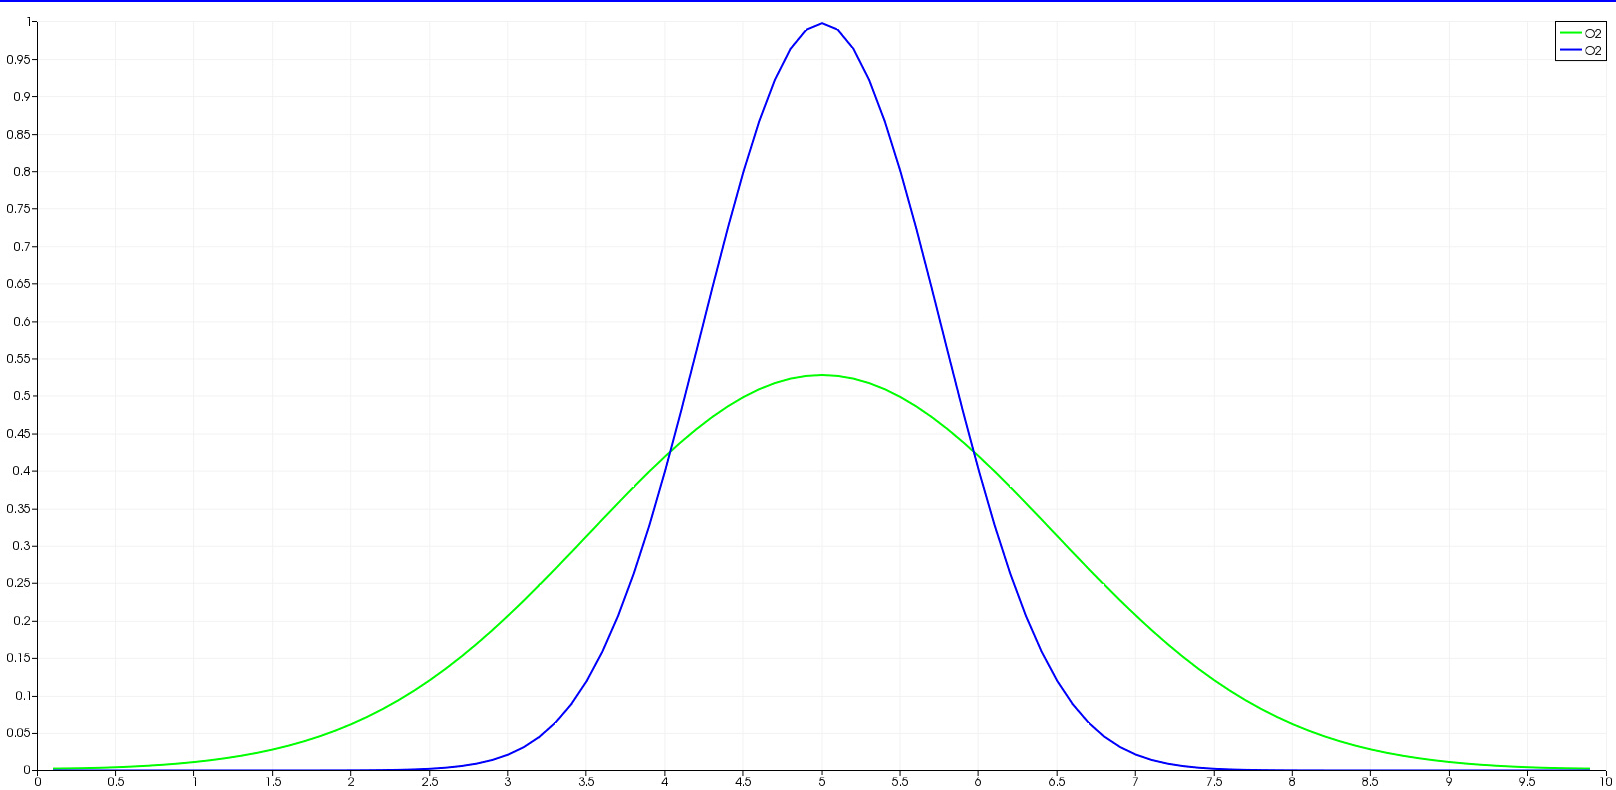
\includegraphics[width=.9\linewidth]{figures/diff.png}
%    \caption{\label{fig:diff_0}Valeur x $t_0$}
%  \end{minipage}%
%  \begin{minipage}{.5\textwidth}
%    \centering
%    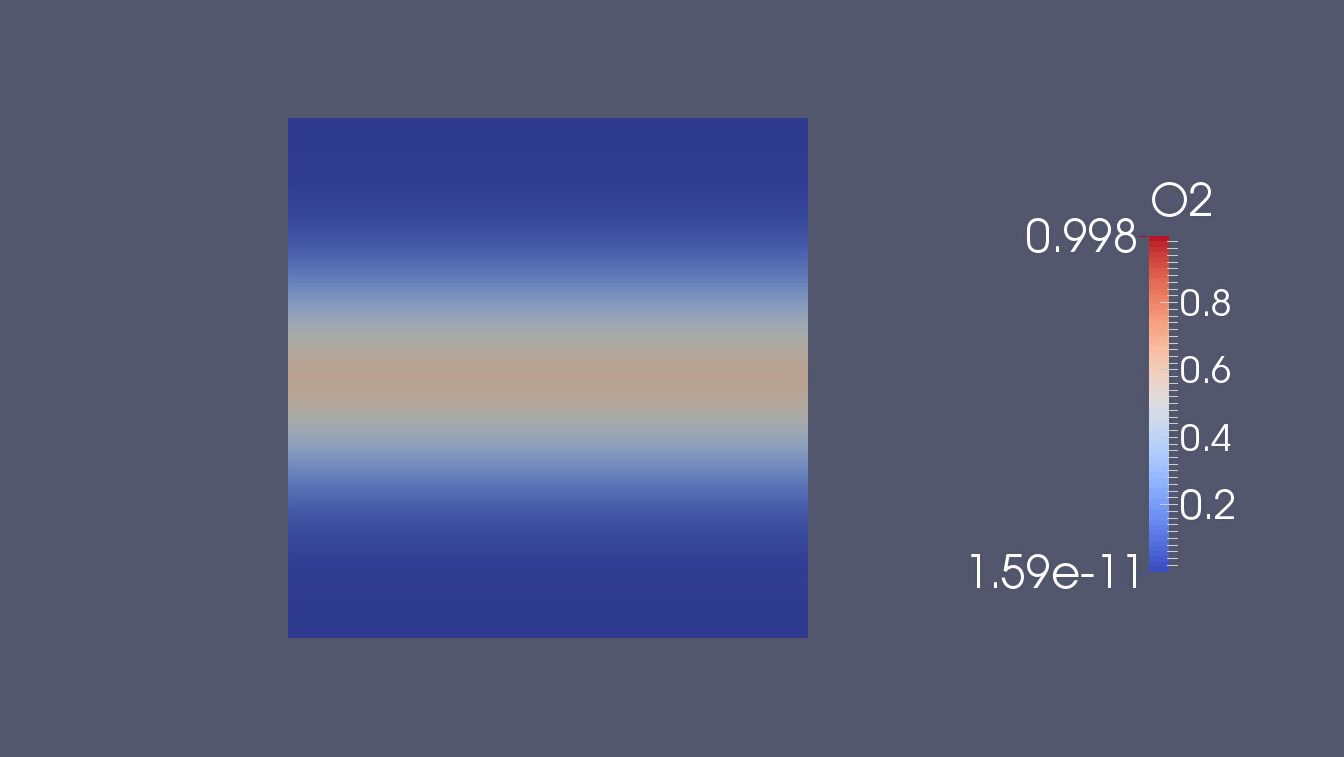
\includegraphics[width=.9\linewidth]{figures/diff_325.png}
%    \caption{\label{fig:diff_325}Valeur x $t$}
%  \end{minipage}
%  \centering
%  \begin{minipage}{.5\textwidth}
%    \centering
%    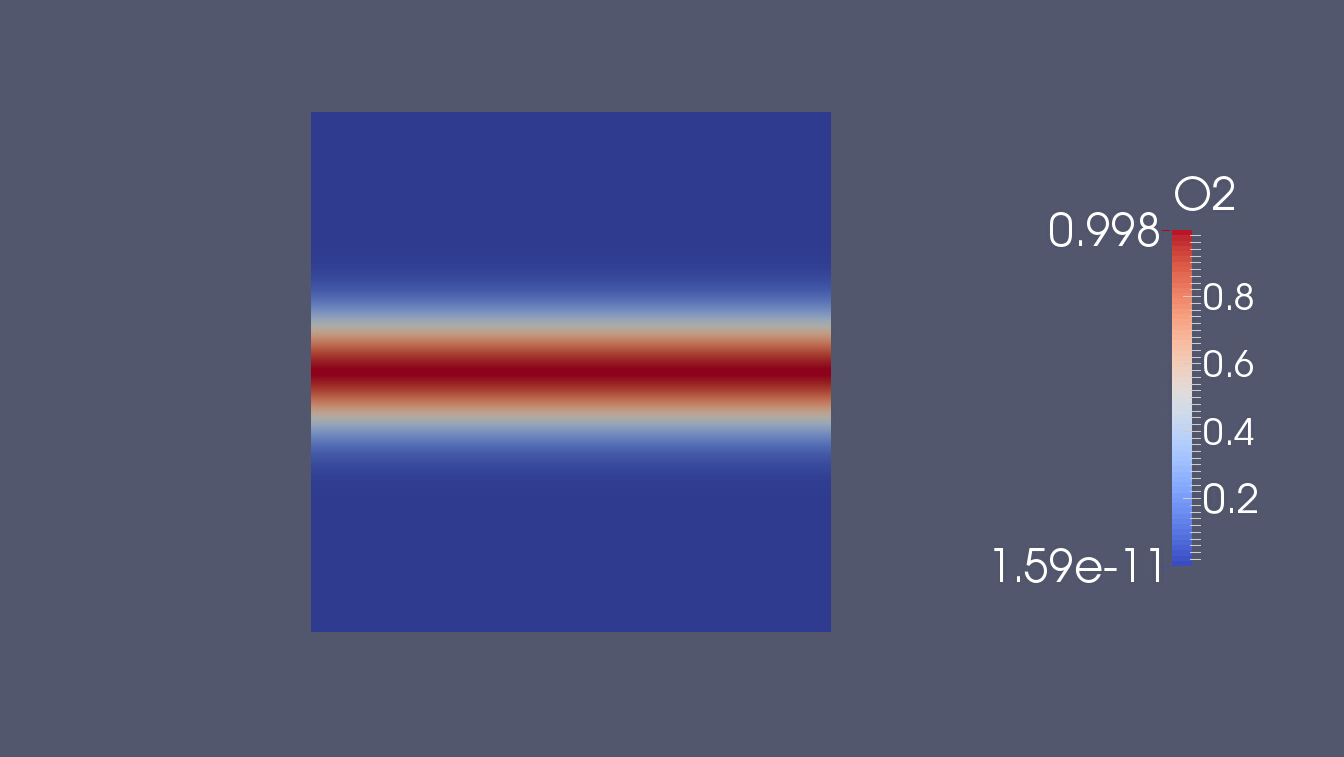
\includegraphics[width=.9\linewidth]{figures/diff_0.png}
%    \caption{\label{fig:diff_0_domain}Valeur x $t_0$ - Domaine complet}
%  \end{minipage}%
%  \begin{minipage}{.5\textwidth}
%    \centering
%    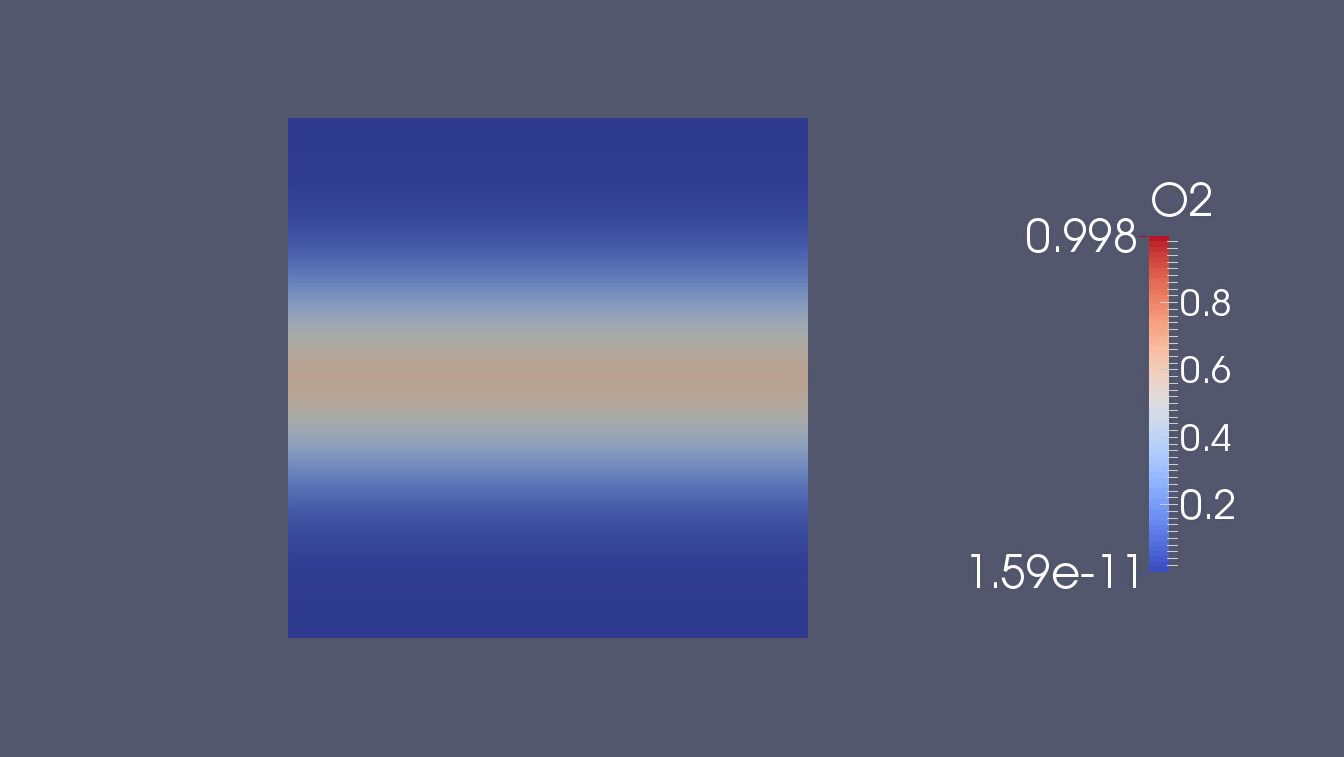
\includegraphics[width=.9\linewidth]{figures/diff_325.png}
%    \caption{\label{fig:diff_325_domain}Valeur x $t$ - Domaine complet}
%  \end{minipage}
%  \caption{\label{fig:diff_}Diffusion}
%\end{figure}


\paragraph{Turbulence homogène isotrope}
(help bénédicte)

\begin{figure}[ht]
  \centering
  %\includegraphics[scale=0.3]{figures/turbiso.png}
  \caption{\label{fig:turbiso}Turbulence homogène isotrope}
\end{figure}




\cleardoublepage
\section{Partie 2:Parallélisation de NTMIX}

\subsection{Décomposition de domaine}
Comme vu dans l'introduction, l'objectif est de pouvoir faire tourner cette application sur un maillage de taille conséquente ($\approx 10^9$ points). Pour cela, MPI sera utilisé plutôt que OpenMP. En effet, l'approche mémoire partagée oblige à avoir l'ensemble de la mémoire utilisée par l'application au même endroit, hors pour $10^9$ points, la mémoire nécessaire est de l'ordre de 120 Gigaoctets. Les supercalculateurs ne possédant pas autant de mémoire, l'approche MPI paraît plus satisfaisante; chaque processus stockera une partie du domaine ce qui reduira l'utilisation de mémoire.

\paragraph{}Pour cela, il est possible avec MPI de disposer les processus sur une grille cartesienne.
Le but est de diviser le domaine de calcul entre plusieurs processus, chacun calculant ainsi une portion du problème. Cependant, chaque processus ne peut pas travailler de manière totalement indépendante, il est nécessaire d'introduire des points de synchronisations afin que des échanges d'informations se mettent en place: 

\paragraph{}Il sera donc nécessaire d'introduire des points de synchronisation dans l'application; pour l'opération de réduction du pas de temps et pour l'échange des données servant à remplir l'overlapping de chacun des processus.

\subsection{Recouvrement de domaine}
\paragraph{} Cependant, chaque processus ne peut pas travailler de manière totalement indépendante. En effet, une méthode compacte est utilisée pour calculer les gradients des diffèrents champs. Une telle méthode implique que le gradient en un point est dépendant des valeurs de tous les autres points du champ. Les points se trouvant sur les bordures internes (bordures entre processus) manque donc d'information pour réaliser des calculs précis. Pour résoudre ce problème, il est nécessaire d'agrandir artificiellement les sous-domaines de chaque processus afin qu'ils ``débordent'' sur les sous-domaines voisins (overlapping). Sur la figure \ref{fig:overlap}, on peut voir que le domaine est divisé selon les pointillés rouge; ils représentent les parties du domaine réellement calculés par les différents processus. Les lignes bleues représentent l'overlapping des différents processus


\begin{figure}[t!]
  \centering
  \begin{subfigure}[b]{0.5\textwidth}
    \centering
    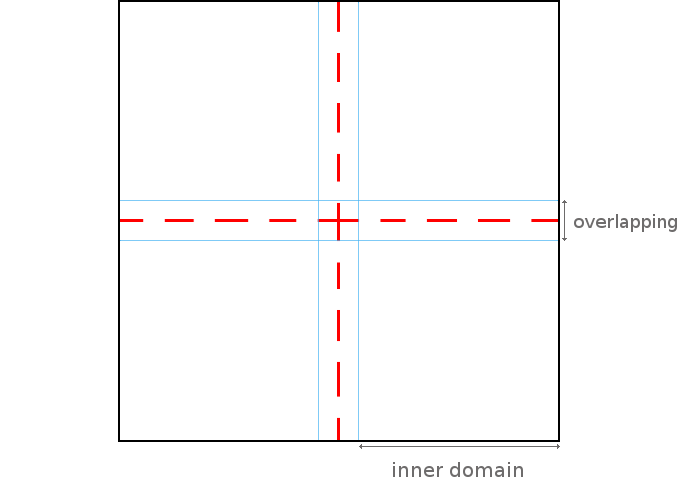
\includegraphics[scale=0.3]{figures/domain_overlap.png}
    \caption{\label{fig:overlap_domain}Représentation de l'overlapping - Domaine}
  \end{subfigure}%
  ~ 
  \begin{subfigure}[b]{0.5\textwidth}
    \centering
    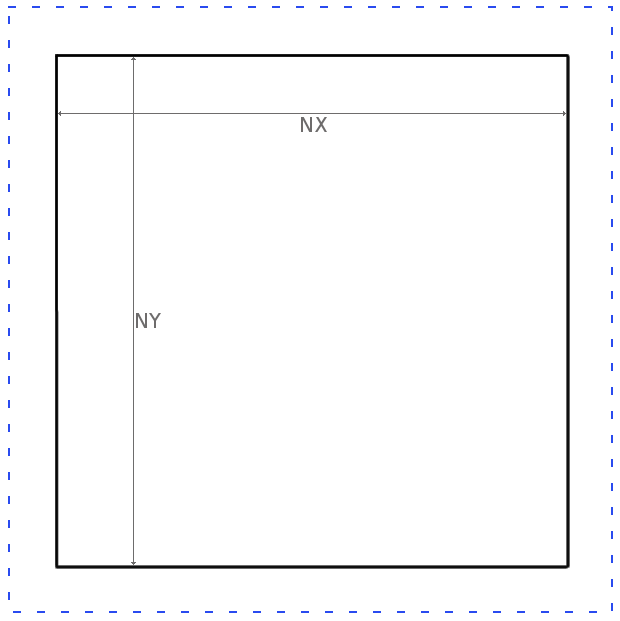
\includegraphics[scale=0.3]{figures/overlap.png}
    \caption{\label{fig:overlap_subdomain}Représentation de l'overlapping - Sous-domaine}
  \end{subfigure}
  \caption{\label{fig:overlap}Diffusion}
\end{figure}
% NX et NY représente la taille du domaine de validité d'un processus. Les pointillés bleus représente cet overlapping qui contiendra les valeurs des domaines adjacents.

L'exactitude des résultats dépendra donc de la taille de cet overlapping, c'est pour cela que le choix sera laissé à l'utilisateur même si une étude sera présenté.



\subsubsection{Méthode d'overlapping}
En pratique, il existe 2 méthode pour réaliser l'overlapping présenté précedemment, elles diffèrent seuleument dans le moment auquel les communications entre les processus seront réalisées. Mais l'idée générale reste la même. Les données permettant de calculer les gradients du sous-domaine d'un processus se trouvent sur ses processus voisins. On peut donc créer des ``cellules fantômes'' autour du sous-domaine qui contiendront les valeurs requises. Sur la figure \ref{fig:neighbor_buf}, on peut voir en orange les ``cellules fantômes'' qui recevront les valeurs voisines et en vert les valeurs qui seront envoyées aux processus voisins. 

\begin{figure}[h]
  \centering
  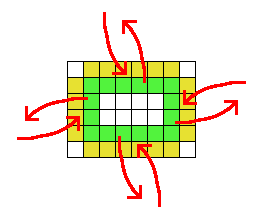
\includegraphics[scale=1]{figures/domain_overlap2.png}
  \caption{\label{fig:neighbor_buf}Motif de communication d'un processus}
\end{figure}


%\begin{figure}[h]
%  \centering
%  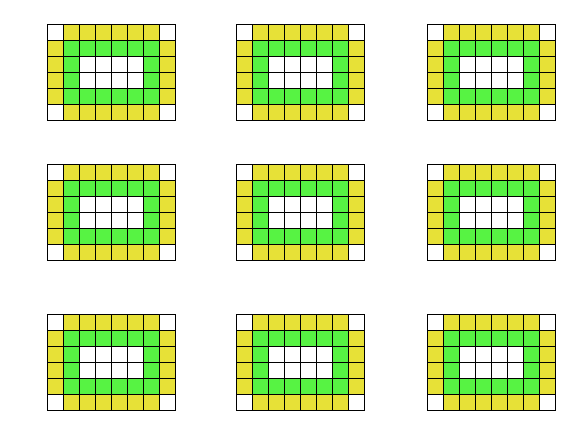
\includegraphics[scale=0.5]{figures/halo.png}
%  \caption{\label{fig:neighbor_buf} Motif de communication}
%\end{figure}

\paragraph{}Une méthode de Runge-Kutta est utilisée lors du calcul de l'avancé du temps. C'est une méthode d'analyse numérique permettant l'approximation de solutions d'équations différentielles. Elle est réalisé en 3 étapes (algo \ref{}) et dans chacune de ces étapes des gradients sont calculés.

\begin{algorithm}
  \caption{Time loop}
  \label{algo:time_loop}
  \begin{algorithmic}
     \FOR{time<final\_time} 
     \STATE {Call compute\_timestep} 
     \STATE {Call time\_step}
     \ENDFOR
  \end{algorithmic}
\end{algorithm}

\begin{algorithm}
  \caption{time\_step}
  \label{algo:time_step}
  \begin{algorithmic}
     \FOR{time<final\_time} 
     \STATE {Call RHS(1)} 
     \STATE {Call impose\_boundary\_conditions}
     \STATE {Call RHS(2)} 
     \STATE {Call impose\_boundary\_conditions}
     \STATE {Call RHS(3)} 
     \STATE {Call impose\_boundary\_conditions}
     \ENDFOR
  \end{algorithmic}
\end{algorithm}

\paragraph{1ère méthode}Cette première méthode consiste à réaliser les communications avant chaque appel à RHS. Ainsi, la région d'overlapping possède les valeurs calculées par les voisins et peuvent être utilisées pour les calculs locaux de gradient. Avec cette méthode, 3 grandes communications sont réalisées par pas de temps.

\paragraph{2éme méthode}Dans cette seconde méthode, un processus récupère les valeurs d'une seule variable conservative au moment du calcul du gradient correspondant. Cette fois-ci, les communicattions sont plus nombreuses et plus petites. 

%\paragraph{1ère méthode}Cette première méthode consiste à récupérer la région d'overlapping pour chaque variable conservative en début du pas de temps, avant tout calcul de gradient. L'évolution de ces points sera calculée et ils seront ensuite utilisés lors du calcul des gradients sur les différents champs. Avec cette méthode, une seule communication est réalisée par pas de temps mais le coût des calculs et du stockage est augmenté.


\paragraph{}J'ai donc ajouter ces méthodes au programme pour pouvoir comparer leurs performances respectives. La première méthode à l'avantage de reduiré la fréquence des communications en dupliquant des calculs sur plusieurs processus (augmentant donc le côut de ceux-ci).


\paragraph{}Dans la version séquentielle, un pas de temps maximal est calculé dans le but d'assurer la stabilité de l'algorithme. Ce calcul est donc dépendant de l'ensemble du domaine. Dans la version parallèle, chaque processus devra donc calculer le pas de temps maximal de son sous-domaine et le communiquer aux autres afin de trouver le pas de temps global (opération de réduction).

% \begin{itemize}
% \item pour le calcul du pas de temps; dans la version séquentielle, un pas de temps maximal est calculé dans le but d'assurer la stabilité de l'algorithme. Dans la version parallèle, chaque processeur devra donc calculer le pas de temps maximal de son sous-domaine et le communiquer aux autres afin de trouver le pas de temps global (opération de réduction).
% \item pour le calcul des gradients; une méthode compacte est utilisée pour calculer les gradients des différents champs. Une telle méthode implique que le gradient en un point est dépendante de tous les autres points du domaine. Il sera donc nécessaire d'échanger des informations entre les processus pour ce calcul reste juste.
% \end{itemize}



\subsection{Equilibrage de charge}
Lors d'un tel découpage de domaine, il est nécessaire de s'assurer que la quantité de travail réalisée par chaque processus est semblable à celle des autres. Le but est donc de distribuer le même nombre de mailles sur chaque processus. Dans le cas d'un domaine périodique ce problème n'apparaît pas car chaque processus possédent des regions d'overlapping dans toutes les directions. Cependant, si le domaine possède des frontières physique (cas symmétrique), certains sous-domaines n'auront pas le même besoin d'overlapping.

\paragraph{}Prenons l'exemple d'un domaine de 100x100x100 répartis sur une grille de 4x4x4 processus avec un overlapping de 4: si on découpe le domaine de manière triviale, on obtient donc 64 sous-domaines de taille 25x25x25. Si on ajoute ensuite les points d'overlapping, on retrouve 4 classes de sous-domaines ayant des tailles différentes (fig. \ref{fig:domain_desequilibre}); les coins du domaine auront donc 30x30x30 points, les autres sous-domaines situés sur les bordures physique auront 35x30x30 points, les sous-domaines situés sur les faces externes 35x35x30 et tous les autres 35x35x35. Comme on peut le constater dans le tableau \ref{arr:overlap_res}, la charge de calcul est désiquilibrée entre les processus et certain processus (ceux ayant le moins de travail) devront atteindre les autres pour les synchronisations présentées en début de partie. Même si ce comportement est moins marqué lorsque les sous-domaines sont plus grands (\ref{arr:overlap_res_big}), il est préférable de l'éviter.
  
Si on ajoute la taille totale de l'overlapping avant de découper le domaine, les tailles des domaines internes varient selon les processus mais la taille globale (domaine interne + overlapping) est identique. Toujours avec l'exemple précédent, si on ajoute la taille de l'overlapping à la taille globale, on obtient un domaine global de 124x124x124 points. On divise ensuite ce domaine entre les processus et on obtient cette fois-ci une seule classe de sous-domaines de 31x31x31 points. On joue ici sur la taille du domaine interne pour équilibrer la charge. Un sous-domaine se trouvant sur un coin aura un domaine interne de 27x27x27 alors qu'un sous-domaine de classe A aura 23x23x23 point sur son domaine interne.


\begin{figure}[ht]
  \centering
  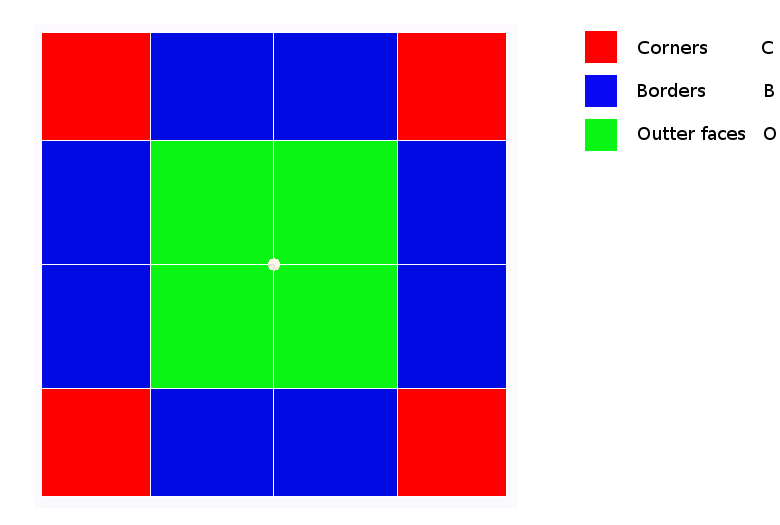
\includegraphics[scale=0.3]{figures/domain_dese.png}
  \caption{\label{fig:domain_desequilibre}Exemple de déséquilibre de charge}
\end{figure}

\begin{table}[h]
  \begin{center}
    \begin{tabular}{|P{2cm}|P{3.5cm}|P{3.5cm}|}
      \hline
      & Taille & Overhead \\ \hline
      C & 29x29x29 & 0\%  \\ \hline
      B & 33x29x29 & 13.8\%  \\ \hline
      F & 33x33x29 & 29.5\%  \\ \hline
      A & 33x33x33 & 47.3\%  \\ \hline      
    \end{tabular}
    \caption{\label{arr:overlap_res}Surcout de calcul - 100x100x100, 64 processus, overlapping 4}
  \end{center}
\end{table}


\begin{table}[h]
  \begin{center}
    \begin{tabular}{|P{2cm}|P{3.5cm}|P{3.5cm}|}
      \hline
      & Taille & Overhead \\ \hline
      C & 205x205x205 & 0\%    \\ \hline
      B & 210x205x205 & 2.4\%  \\ \hline
      F & 210x210x205 & 4.9\%  \\ \hline
      A & 210x210x210 & 7.5\%  \\ \hline      
    \end{tabular}
    \caption{\label{arr:overlap_res_big}Surcout de calcul - 1000x1000x1000, 125 processus, overlapping 5}
  \end{center}
\end{table}


\paragraph{}Un déséquilibre de charge peut également apparaître lors de la phase d'initialisation, même si son impact est failble, il est préférable de l'éviter. En effet, il faut éviter qu'un seul processus doive initialiser l'ensemble du domaine puis envoyer les informations calculées à tous les autres processus. Dans le cas de ce programme l'initialisation peut-être réalisée de manière indépendante (sans aucune synchronisaton). En effet, les initialisations simples (valeur d'une variable fournies dans le fichier de configuration) ne nécessite aucun calcul. Les initialisation nécessitant des calculs sont en général basée sur la position physique des point du domaines et peuvent donc être initialisés en totale indépendances, le plus souvent par une fonction.

\subsection{Communications}Je m'intéresse ici aux méthodes de communications utilisées dans la première méthode présentée ci-dessus. En effet la seconde méthode d'overlapping n'induit qu'au plus 2 communications par processus par calcul de gradients et ne pose donc pas de problèmes particuliers. En revanche, pour la première méthode il faut effectuer au plus 2x3 communications par appel à la fonction update. J'ai testé plusieurs de communications pour comparer leurs performance. J'ai dans un premier temps utilisé la fonction MPI\_Neighbor\_alltoallv. Pour l'utiliser, il faut préparer un buffer qui contiendra les données à envoyer à chacun de ses voisins(fig. \ref{fig:neighbor_pos}). La fonction s'occupe elle-même d'envoyer la bonne partie du buffer au bon voisin selon leur disposition sur la grille cartésienne. Après l'appel à cette fonction, le buffer de réception contient les données de tous les voisins autour d'un processus. Il ne reste plus qu'à stocker les variables reçues à leur place. 

\begin{figure}[h!]
  \centering
  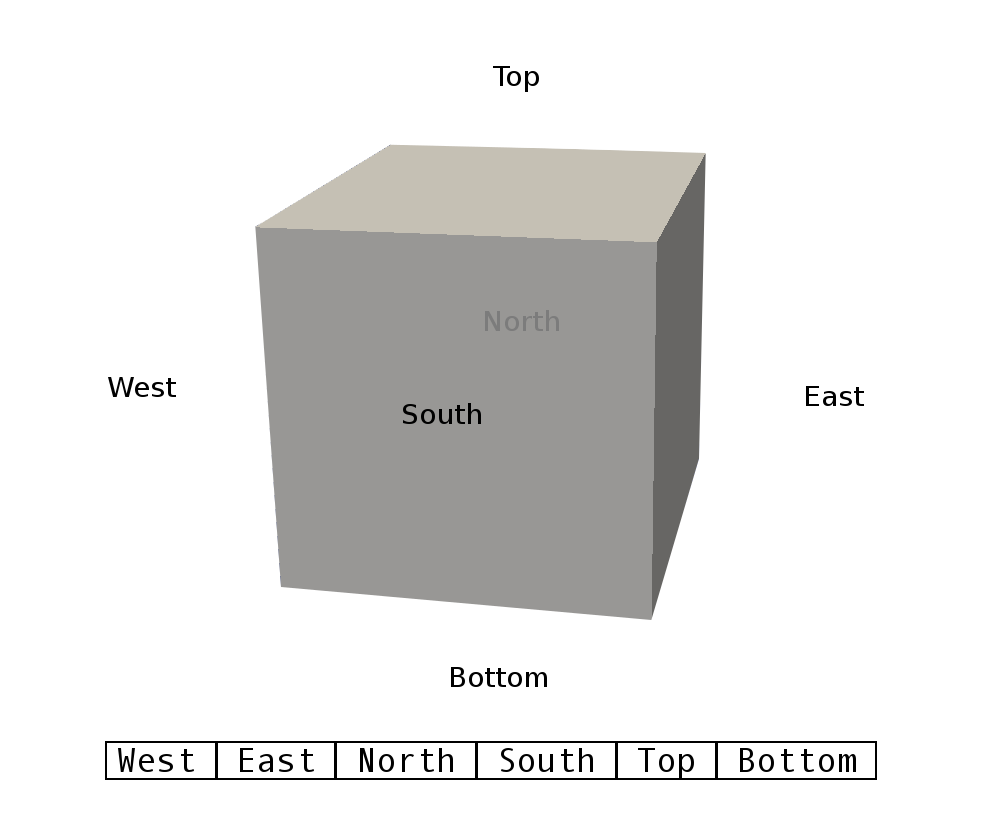
\includegraphics[scale=0.3]{figures/neighbor_pos.png}
  \caption{\label{fig:neighbor_pos}Positions des valeurs des voisins}
\end{figure}

\paragraph{}Cependant cette fonction est relativement récente et peut ne pas être disponible sur certain calculateur qui seront utilisé. Il m'a donc été demandé d'implémenter une seconde méthode dans un soucis de portabilité. C'est une implémentation triviale de la fonction MPI\_Neighbor\_alltoallv; on parcourt les dimensions du domaines, et pour chaque dimensions, on effectue 2 envois et 2 réceptions.

\paragraph{}Le coût d'une telle méthode ne se résume donc pas simplement aux coûts de communications mais aussi aux nombreuses copies réalisées pour créer le buffer d'envoi et pour ``eclater'' le buffer de reception. Ce coût sera donc étudié dans la partie suivante.

\subsection{Validation}

\paragraph{Cas d'un unique processus}Avant de tester la validité du programme avec plusieurs processus, il est nécessaire de s'assurer qu'il peut être lancé avec un seul processus et que les résulats fournis soient exactement identiques à la version 3D validée à la section \ref{sec:3D-validation}. Même si ce test paraît trivial, il est important de le faire. Il sera également utile de comparer le temps pris par ce test par rapport au temps de la version 3D séquentielle pour estimer le surcôut pouvant être induit par l'utilisation de MPI (découpage du domaine, calcul de l'overlapping, fausses communications ...).

\paragraph{Cas avec décomposition de domaine}
Comme vu dans la section \ref{sec:p2-tr} le calcul des gradients est dépendant de l'ensemble du domaine. Pour s'assurer de l'exactitude des résultats obtenus dans cette version MPI, j'ai donc utiliser un overlapping assez grand permettant d'affiner les résultats au maximum. J'ai ensuite calculer les valeurs moyennes des champs de la solution afin de les comparer avec ceux obtenus avec la version séquentielle du programme (\ref{sec:3D-validation}).

\begin{table}[h]
  \begin{center}
    \begin{tabular}{|c|c|c||c|c|c|c||c|c|c|}
      \hline
      Overlap & 12 & 11 \\
      \hline
      Mean error & 10E-14 & 10E-10 \\
      \hline
    
    \end{tabular}
    \caption{\label{arr:overlap_res} Résultats obtenus}
  \end{center}
\end{table}

\cleardoublepage
\section{Partie 3:Etude de performance et optimisations}
\paragraph{}Je me suis finalement penché sur les performances de la version 3D de NTMIX développé au cours de ce stage. J'ai dans un premier temps étudié les performances séquentielles du programme (code tel qu'il était à la fin de la première partie) puis les performances de la version parallèle.
\subsection{Présentation du matériel}
L'ensemble des tests suivants ont été réalisés sur les calculateurs internes du CERFACS, le Bullx B510 (neptune) et le LENOVO (nemo). Ils possèdent les caractéristiques suivantes:

\begin{table}[h]
  \begin{center}
    \begin{tabular}{|M{3.5cm}|M{5cm}|M{5cm}|}
      \hline
      & Neptune & Nemo \\
      \hline
      Noeuds & 158 & 252 \\
      \hline
      Puissance crête & 53 TFlop/s & 242 TFlop/s \\
      \hline
      Consommation maximale applicative & 51 kW.h & 73 kW.h \\
      \hline
      Consommation à vide & 25 kW.h & 34 kW.h \\
      \hline
      Processeurs & Intel Sandy Bridge 8 coeurs (2.6 GHz) & Intel Ivy bridge 12 coeurs (2.5 GHz) \\
      \hline
      Mémoire & 32 Go de mémoire cadencée à 1.6 GHz & 64 Go de mémoire cadencée à 2.1 GHz \\
      \hline
    \end{tabular}
  \end{center}
  \caption{\label{tab:carac}Caractèristiques des calculateurs du Cerfacs}
\end{table}

\begin{figure}[ht]
  \centering
  \begin{minipage}{.5\textwidth}
    \centering
    \includegraphics[width=.7\linewidth]{figures/neptune.jpg}
    \caption{\label{fig:neptune}Neptune}
  \end{minipage}%
  \begin{minipage}{.5\textwidth}
    \centering
    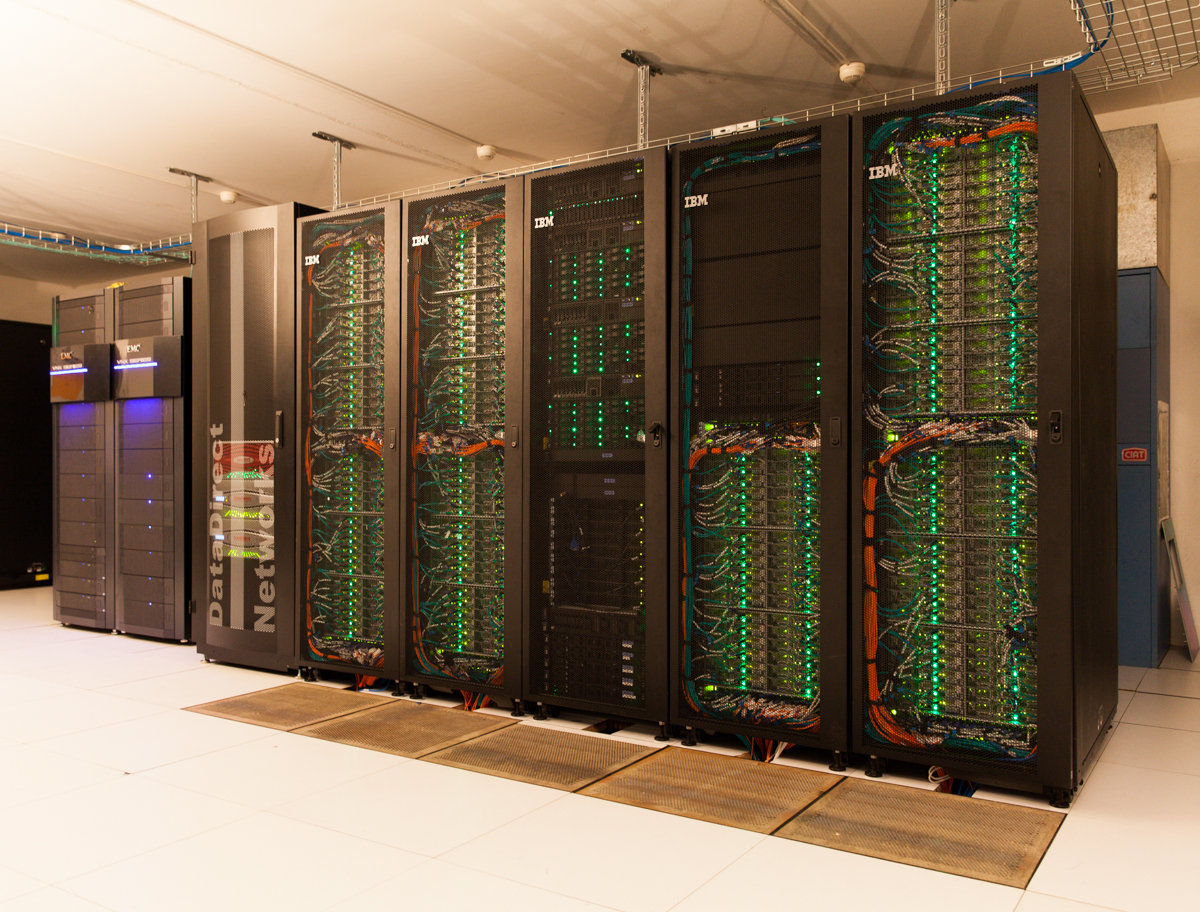
\includegraphics[width=.9\linewidth]{figures/nemo.jpg}
    \caption{\label{fig:neptune_node}Nemo}
  \end{minipage}
\end{figure}



\subsection{Performances séquentielles}
Une fois le programme testé et fonctionnel, j'ai commencé à étudier ses performances. J'ai, dans un premier temps, mesuré un temps de référence pour l'exécution de ce programme; compilation par défaut, donc avec l'option -O2.

\subsubsection{Vectorisation}
J'ai ensuite compiler le programme avec l'option -xAVX qui permet de générer un code vectorisé pour les processeurs possédant l'extension AVX. Pour profiler le programme, j'ai utilisé Intel Advisor qui permet d'analyser la vectorisation d'un programme. Comme on peut le constater sur la figure \ref{fig:advixe}, le compilateur n'a vectorisé qu'un faible pourcentage de boucles (en comparaison avec la référence cf img). Ceci vient du fait que l'ensemble des variables sont contenues dans un unique tableau (fig. \ref{fig:array_s}) et qu'on y accède grâce à des pointeurs. Lorsqu'une boucle doit travailler sur plusieurs tableaux contenus dans ce grand tableau (fig. \ref{fig:o2_avx_novect}), le compilateur assume qu'elle travaille sur un unique grand tableau et empêche donc la vectorisation au profit de la cohérence. Pour résoudre ce problème, il suffit d'indiquer au compilateur qu'il n'y a pas aliasing; on garantit ainsi qu'une zone mémoire ne peut être accédée que par un nom et que le programme ne dépassera pas les limites d'un tableau.


\begin{figure}	
  \centering
  \begin{minipage}{.5\textwidth}
    \centering
    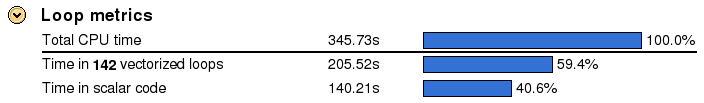
\includegraphics[width=.9\linewidth]{figures/advixe_O2.png}
    \caption{\label{fig:advixe_o2}}
  \end{minipage}%
  \begin{minipage}{.5\textwidth}
    \centering
    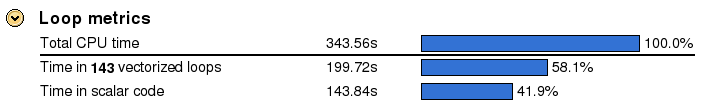
\includegraphics[width=.9\linewidth]{figures/advixe_O2_avx.png}
    \caption{\label{fig:advixe_o2_avx}Caption 2}
  \end{minipage}
  \caption{Répartition des boucles}\label{fig:advixe}
\end{figure}

\begin{figure}[ht]
  \centering
  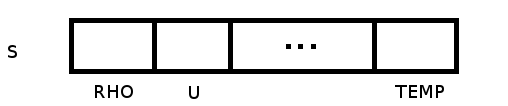
\includegraphics[scale=0.35]{figures/array_s.png}
  \caption{\label{fig:array_s}Structure de la mémoire}
\end{figure}


\begin{figure}[h]
  \centering
  \begin{lstlisting}
    !
    !    DETERMINE THE MASS FRACTION
    !
    DO I=1,NX*NY*NZ
    YK(I)=RHO_Y_TILDE(I,K)/RHO(I)
    END DO
  \end{lstlisting}
  \caption{\label{fig:o2_avx_novect}Boucle non vectorisée}
\end{figure}



\begin{figure}	
  \centering
  \begin{minipage}{.5\textwidth}
    \centering
    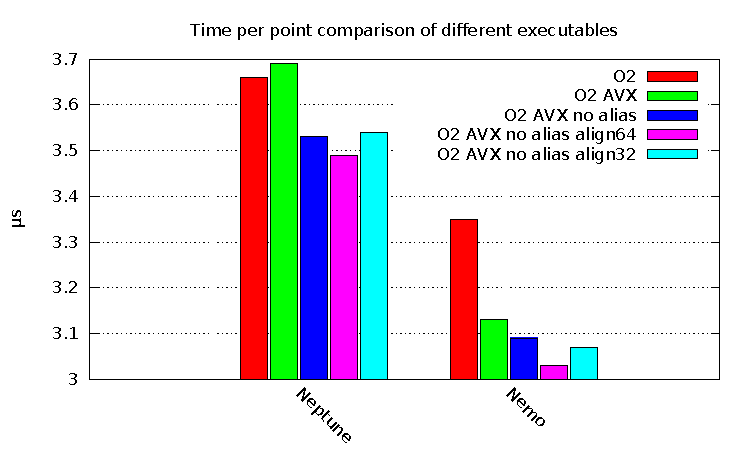
\includegraphics[width=.9\linewidth]{gnuplot/bench_scalaire_per_compute.pdf}
  \end{minipage}%
  \begin{minipage}{.5\textwidth}
    \centering
    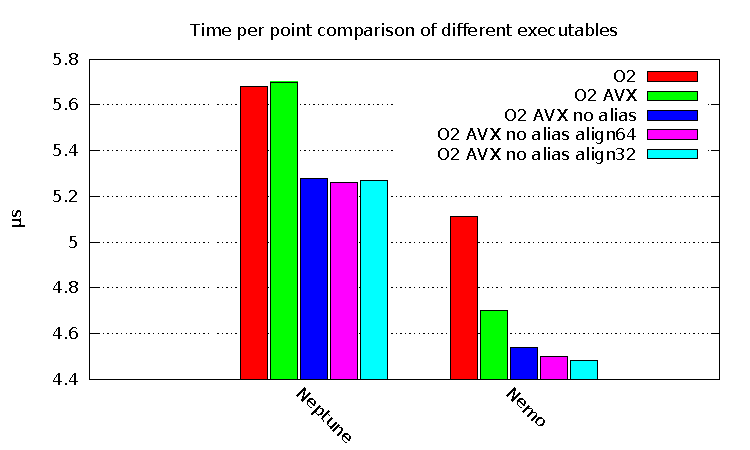
\includegraphics[width=.9\linewidth]{gnuplot/bench_scalaire_per_diag.pdf}
  \end{minipage}
  \caption{Temps par point - Cas périodique}\label{fig:scal_tpp}
\end{figure}


\begin{figure}	
  \centering
  \begin{minipage}{.5\textwidth}
    \centering
    % \includegraphics[width=.9\linewidth]{gnuplot/bench_scalaire_sym_compute.pdf}
    \caption{\label{fig:scal_compute}}
  \end{minipage}%
  \begin{minipage}{.5\textwidth}
    \centering
    % \includegraphics[width=.9\linewidth]{gnuplot/bench_scalaire_sym_diag.pdf}
    \caption{\label{fig:scal_diag}Caption 2}
  \end{minipage}
  \caption{Temps par point - Cas symétrique}\label{fig:scal_tpp}
\end{figure}



\subsubsection{Alignement de la mémoire}
blabla marche pas

\paragraph{durée=f(taille)}


\subsection{Performances parallèle}

\subsubsection{Méthode de recouvrement}



\subsubsection{Méthode de communication}

\cleardoublepage
\section*{Conclusion}\addcontentsline{toc}{section}{Conclusion}

\appendix

\section{NSCBC: Navier-Stokes Characteristic Boundary Conditions}\label{app:nscbc}

Ces équations décrivent les ondes utilisées dans la méthode \textit{NSCBC}, implémentées pour la version tridimensionnelle de NTMIX. 


\begin{subequations}
\begin{align}
  \begin{split}
    \mathcal{L}_1&=(u-c)\left[ \left( \frac{1}{2} \frac{\gamma -1}{\gamma} \frac{T}{\rho} \right) \frac{\partial \rho}{\partial x} + \left( \frac{1}{2} \frac{\gamma -1}{\gamma} \right) \frac{\partial T}{\partial x}  -  \left( \frac{1}{2} \frac{c}{\overline{C}_p}  \right) \frac{\partial u}{\partial x} \right.\\
      &\left. + \sum_{i=1}^{N_s} \left(  \frac{1}{2} \frac{\gamma -1}{\gamma} \frac{\overline{W}T}{W_i} \right) \frac{\partial Y_i}{\partial x}   \right]
  \end{split}\label{eq:l1}\\
~
  \mathcal{L}_2&= u \frac{\partial v}{\partial x}\label{eq:l2}\\
~
  \mathcal{L}_3&= u \frac{\partial w}{\partial x}\label{eq:l3}\\
~
  \begin{split}
    \mathcal{L}_4&=u \left[ \left( \frac{1- \gamma}{\gamma} \frac{T}{\rho} \right) \frac{\partial \rho}{\partial x} + \left( \frac{1}{\gamma} \right) \frac{\partial T}{\partial x} - \left( \frac{\overline{W}T}{W_1} \right) \frac{\partial Y_1}{\partial x} \right. \\
      &\left. + \sum_{i=1}^{N_s} \left(  \frac{1}{\gamma} \frac{\overline{W}T}{W_i} \right) \frac{\partial Y_i}{\partial x}  \right]
    \end{split}\\
~
  \mathcal{L}_{j+3}&=u  \left[ - \left( \frac{\overline{W}T}{W_j} \right) \frac{\partial Y_j}{\partial x} \right]\\
~
  \mathcal{L}_{N_s+4}&=u \left[ \left( \frac{\gamma -1}{\gamma} \right) \frac{\partial \rho}{\partial x} - \left( \frac{\rho}{\gamma T} \right) \frac{\partial T}{\partial x} - \sum_{i=1}^{N_s} \left(  \frac{\overline{W}}{W_i} \frac{\rho}{\gamma} \right) \frac{\partial Y_i}{\partial x}  \right]\\
~
  \begin{split}
    \mathcal{L}_{N_s+5}&=(u+c)\left[ \left( \frac{1}{2} \frac{\gamma -1}{\gamma} \frac{T}{\rho} \right) \frac{\partial \rho}{\partial x} + \left( \frac{1}{2} \frac{\gamma -1}{\gamma} \right) \frac{\partial T}{\partial x}  +  \left( \frac{1}{2} \frac{c}{\overline{C}_p}  \right) \frac{\partial u}{\partial x} \right.\\
      &\left. + \sum_{i=1}^{N_s} \left(  \frac{1}{2} \frac{\gamma -1}{\gamma} \frac{\overline{W}T}{W_i} \right) \frac{\partial Y_i}{\partial x}   \right]
  \end{split}\label{eq:llast}
\end{align}
\end{subequations}




\newpage
\section{Résultats des performances séquentielles sur le calculateur Bullx}\label{app:seq_neptune}

Cette annexe présente les obtenus par la méthode décrite en section \ref{fig:vecto} sur le second calculateur du Cerfacs.

\begin{figure}[!ht]
  \centering
  \begin{subfigure}[b]{0.5\textwidth}
    \centering
    \includegraphics[page=1,scale=0.51]{gnuplot/bench_scalaire_neptune.pdf}
  \caption{\label{fig:bench_scal_neptune_nonper}}
  \end{subfigure}%
  ~
  \begin{subfigure}[b]{0.5\textwidth}
    \centering
    \includegraphics[page=2,scale=0.51]{gnuplot/bench_scalaire_neptune.pdf}
  \caption{\label{fig:bench_scal_neptune_sym}}
  \end{subfigure}
  \begin{subfigure}[b]{0.5\textwidth}
    \centering
    %\includepdf[pages={2}]{gnuplot/bench_scalaire.pdf}
    \includegraphics[page=3,scale=0.51]{gnuplot/bench_scalaire_neptune.pdf}
  \caption{\label{fig:bench_scal_neptune_per}}
  \end{subfigure}
  \caption{\label{fig:bench_scal_neptune}Temps par points des cas tests - BULL}
\end{figure}


%\section{Modifications du traitements des bordures}
%LEs subroutines bc\_x, bc\_y et bc\_z stockaient les plans des bordures selon leur directions respectives. Dans le cas parallèle, un processus ne possédent pas forcément les 2 plans frontières. Ces routines ont donc été modifiées avent de traiter un seul plan et ce grace un argument qui y a été rajouté.
%
%L'appel à ces fonctions dépend donc maintenant de la position du processus sur la grille cartésienne.



\addcontentsline{toc}{section}{Bibliographie}
\bibliographystyle{unsrt}
\bibliography{biblio}
\end{document}
